\chapter{Introduction}\label{introduction}

%%%%%%%%%%%%%%%%%%%%%%%%%%%%%%%%%%%%%%%%%%%%%%%%%%%%%%%%%%%%%%%%%%%%%%%%%%%%%%%%%%%%
% SECTION: Background to the study
%%%%%%%%%%%%%%%%%%%%%%%%%%%%%%%%%%%%%%%%%%%%%%%%%%%%%%%%%%%%%%%%%%%%%%%%%%%%%%%%%%%%
\section{Background to the study}

Human behavioural and anatomical activities are influenced by several internal cycles. Among these internal cycles is the \textbf{circadian rhythm}, a rhythm studied for many years and whose impacts on the human activity have led to new interests in the regulation of these activities. Formally defined as a \say{cyclical changes in hormones, body temperature, and other biological processes over the course of a 24 hour period} \cite{ge2014}, the Natural Institute of Health (NIH) defines it as \say{a physical, mental and behavioural changes that follow a roughly 24-hour cycle, responding primarily to light and darkness in an organism's environment}\cite{ge2014}. The circadian rhythm plays an important role as it also affects the human sleeping and rising pattern. The circadian rhythm is influenced by the production of \textit{melatonin} produced by the \textit{pineal gland} whose activities are dependent on the presence of light on the \textit{retinal-hypothalamic tract}\cite{lig1994}.These studies have shown that the presence of light of specific wavelength at certain period of time during a day can affect the normal sleeping cycle.\\   
According to the NIH, there is a correlation between long-term health problems and sleep disorders \cite{ph2002}. While stress levels and lifestyles affect the sleeping pattern, there is a strong evidence that the human sleep-wake cycle is strongly affected by light. With the invention of the electric light and the recent human exposure to LED screens, humans have more exposure to nocturnal light. Recent researches have shown that the usage of LED technologies at night is linked to sleep deficiency. Blueish light is said to have a huge impact on one of the human internal clock\cite{bl2010}. Sleep deficiency due to inappropriate light exposure can be cured using an optimal light exposure\cite{bl2010}. Researchers were able to quantify, qualify and time the light that is suitable to maintain the natural sleep-wake cycles \cite{cir2014}. With these results, it is possible to create an environment that will follow user specific light requirements needed to treat patients having a sleep disorder.


%%%%%%%%%%%%%%%%%%%%%%%%%%%%%%%%%%%%%%%%%%%%%%%%%%%%%%%%%%%%%%%%%%%%%%%%%%%%%%%%%%%%
% SECTION: Objectives of this study
%%%%%%%%%%%%%%%%%%%%%%%%%%%%%%%%%%%%%%%%%%%%%%%%%%%%%%%%%%%%%%%%%%%%%%%%%%%%%%%%%%%%
\section{Objectives of this study}

\subsection{Problems to be investigated}
This project investigates the feasibility of making a user-friendly embedded system, relatively cheap that could be used as a personal medical device in solving human sleep disorder. This problem envelops the following question:
\begin{itemize}
\item[1] Is this possible to use a programmable light source to emit light of around $460nm$ at $30 lux$?\\
This is the light requirement as mentioned in \cref{scope_and_limitations}.
\item[2] Can an embedded system meeting the light requirement mentioned above be used as a personal medical device?\\
The question focuses on the future use of the device in regulating the human sleep-wake cycle by medical prescription of light requirement.
\end{itemize}

\subsection{Purpose of the study}\label{purpose_of_the_study}
The purpose of this study is to create a device that can be used to regulate the human sleep-wake cycle while being user-friendly and a personalisable digital alarm clock. The product would need to be relatively cheap and have more features than its competitor. Moreover, the device should be able to use user-specific data in the regulation of the sleep-wake cycle.\\
Further objectives \footnote{These are sub-objectives that would be implemented depending on the time available} includes:
\begin{itemize}
\item The use of user-specific medical lighting requirements and patterns to be used a personal medical device supplementing sleeping disorder treatment.
\item Ability to pull events from an online calendar and set these events as alarms.
\item User authentication for onboard screen usage and bluetooth connection  
\end{itemize} 


%%%%%%%%%%%%%%%%%%%%%%%%%%%%%%%%%%%%%%%%%%%%%%%%%%%%%%%%%%%%%%%%%%%%%%%%%%%%%%%%%%%%
% SECTION: Scope and Limitations
%%%%%%%%%%%%%%%%%%%%%%%%%%%%%%%%%%%%%%%%%%%%%%%%%%%%%%%%%%%%%%%%%%%%%%%%%%%%%%%%%%%%
\section{Scope and limitations}\label{scope_and_limitations}

The scope of this project involves the design of an functional embedded system named NeoPixels Sunrise Clock also known as NPSC, capable of producing light of $460nm \pm 10nm$ with an intensity of $30 lux$ as mentioned by the paper \textit{"Action Spectrum for Melatonin Regulation in Humans: Evidence for a Novel Circadian Photoreceptor"}. The code and design artefact repository and a full documentation including a user manual, for anybody who wants to make use of the code design resources, also need to the delivered. Moreover, a description of future use of the device in the study of the effect of light on the circadian rhythm will be required.\\
This project does not study the effect of light on the users. For ethical reasons, the NPSC will not be tested on human subjects in real situations of either waking humans or including lighting to facilitate sleep at night. Instead, the system will be tested based on the recommendation from the research literature.\\
The design and creation of the NPSC are subject to several constraints listed below:
\begin{itemize}
\item \textbf{Time:} The project has a duration of 12 weeks within which the research, design, development, implementation, verification, and report writing need to be done.
\item \textbf{Budget:} The project budget allocation is \textbf{R1000}
\item \textbf{Light:} The NPSC must be able to produce blue light with a wavelength of  $460nm$ while providing enough light to meet the requirement of the research paper and provide a various range of colour for sunrise simulation. These requirements narrow the options for choosing the right light emitters.
\item \textbf{Size:} The NPSC is meant to be a bedside lamp, this implies that it should have a relatively small size to be able to fit on a $50cm*50cm$ bedside table. A volume of $25*25*5cm^3$ is the target volume for the final product.
\end{itemize}


%%%%%%%%%%%%%%%%%%%%%%%%%%%%%%%%%%%%%%%%%%%%%%%%%%%%%%%%%%%%%%%%%%%%%%%%%%%%%%%%%%%%
% SECTION: Plan of Development
%%%%%%%%%%%%%%%%%%%%%%%%%%%%%%%%%%%%%%%%%%%%%%%%%%%%%%%%%%%%%%%%%%%%%%%%%%%%%%%%%%%%
\section{Plan of development}

\subsection{Overview of plan}
The project was broken into sections and subsections with an estimated timeline.\\
The \textit{Gantt Chart} used for this project is shown in \cref{fig:gant}. The project started with the an intensive research on the science related to the human sleeping cycle. The research lead to the design of the NPSC consisting of its hardware and software modules. During the manufacturing process, the software framework of the NPSC was continously improved. The NPSC hardware and software integration were done later after the assembly of the hardware. Finally, the software was improved during the remaining lifetime of the project.
\begin{figure}[ht]
\centering
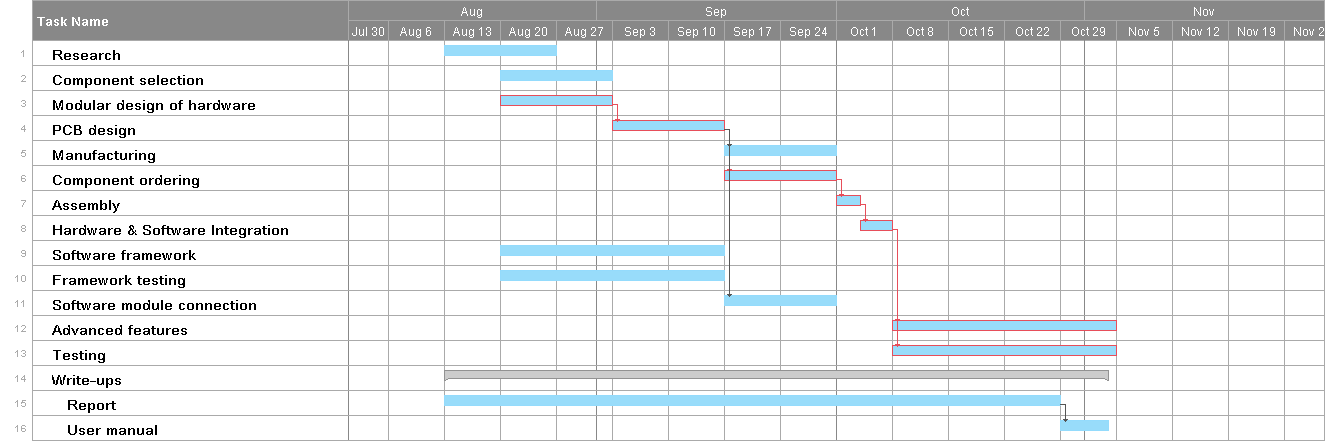
\includegraphics[scale=0.35]{gantt_chart.png}
\caption{Gantt chart showing the timeline of every task in the project as well as its critical path.}
\label{fig:gant}
\end{figure}

\subsection{Chronological progression of the report}
The report organisation is displayed in \cref{fig:wbs}. The sections of the report are explained below:
\begin{itemize}
\item \textbf{Research}
\begin{itemize}
\item \textbf{Introduction:} The feasability of the project as well as its scope and limitations are defined in the introduction. 
\item \textbf{Literature Review:} The literature review gives an insight in the researches made for this project. This includes scientific discoveries on the human sleeping cycle, experiements and results performed  by researchers on that matter, and some technical engineering design decisions. 
\end{itemize} 
\item \textbf{Design} 
\begin{itemize}
\item \textbf{Methodology:} This section covers the hardware, softeare, and mechanical design of the NPSC. 
\item \textbf{Results:} This section displays the results of the hardware and software testing. 
\end{itemize}
\item \textbf{Write-ups} 
\begin{itemize}
\item \textbf{Discussion:} The analysis of the results obtained. Here, the performance of the NPSC is evaluated. A costs and functional analysis of NPSC done to evaluate its performance compared to its competitors. Moreover, the future use of the NPSC is elaborated. 
\item \textbf{Conclusion:} An evaluation of the project, did we achieve the intended goals.
\item \textbf{Recommendations:} We dive into the solutions or recommendations that could improve the design of such device.
\item \textbf{User manual:} This section is for any users of the NPSC. It provides a clear explanation of the features of the NPSC and a detailed manual. 
\end{itemize}
\end{itemize}
\begin{landscape}
\begin{figure}[ht]
\centering
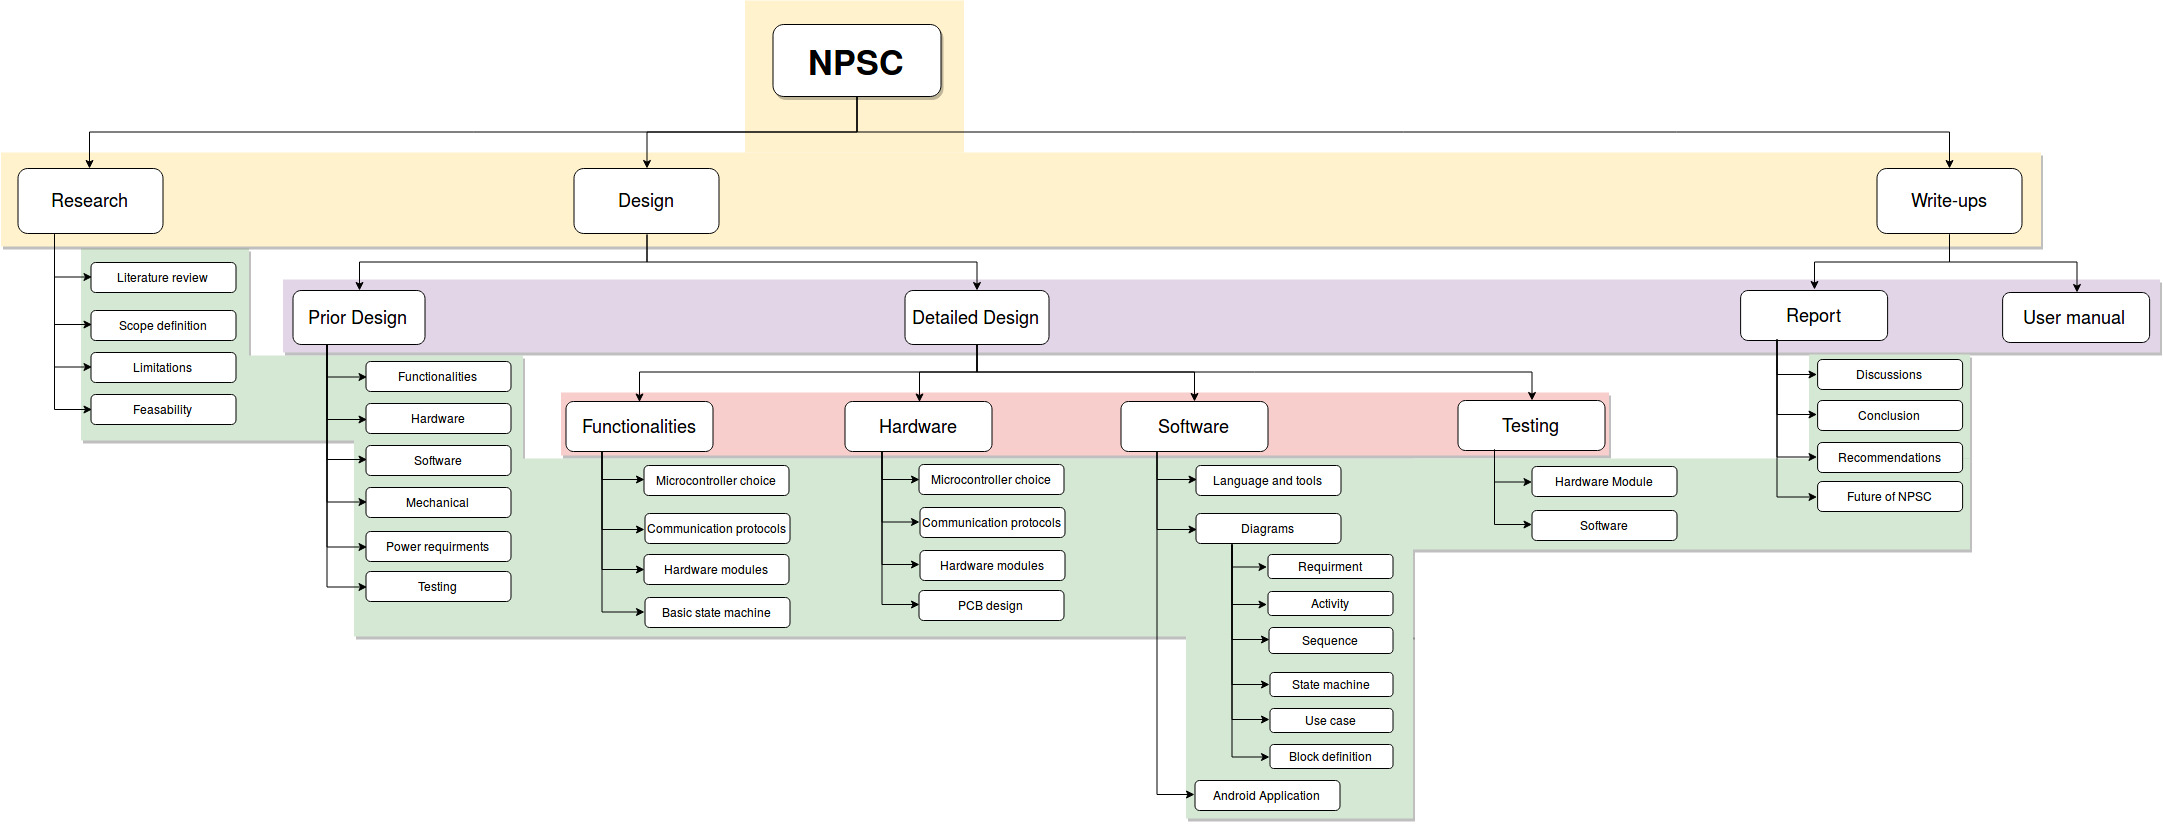
\includegraphics[scale=0.35]{wbs.jpg}
\caption{Report breakdown detailing the different sections needed to be included in the report.}
\label{fig:wbs}
\end{figure}
\end{landscape}
